% Preamble - Parameters of the document
\documentclass[10pt,a4paper]{article}
% Standard packages
\usepackage[utf8]{inputenc}
%\usepackage[italian]{babel}
\usepackage{amsmath}
\usepackage{amsfonts}
\usepackage{amssymb}

\usepackage{graphicx} % Used for pictures
\usepackage[left=2cm,right=2cm,top=2cm,bottom=2cm]{geometry} % Used for margins

\usepackage{listings} % For code source listing
\lstset{language=Python, frame=single} % Listing parameters

\usepackage{hyperref} % Used for external links

% Headers and footers
\usepackage{fancyhdr}
\pagestyle{fancy}
\fancyhf{}
\rfoot{\tiny\textbf{CC-BY-SA}}
\rhead{Pietro Prandini - Stefano Romanello @ UniPD}
\cfoot{\thepage}

% Author and title
\author{Pietro Prandini - Stefano Romanello @ UniPD\\{\textbf{\tiny{CC-BY-SA}}}}
\title{Generation and Analysing Network Attacks using Scapy\\{\small{Project of the Secure Network Management course by DECAMP}}}

% Document
\begin{document}
\maketitle % Shows the title and the authors

\section{The configuration used}
\begin{center}
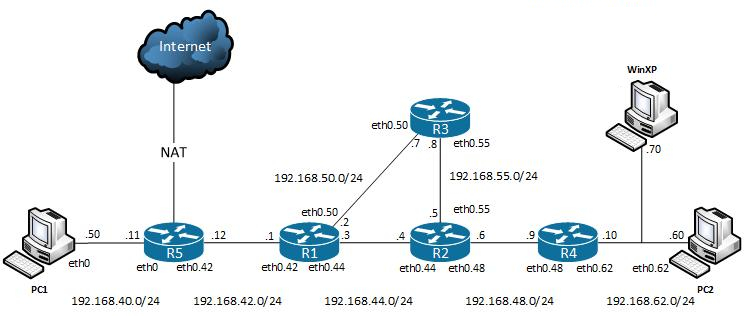
\includegraphics[height=7cm]{img/NetworkConfiguration.jpg}\par
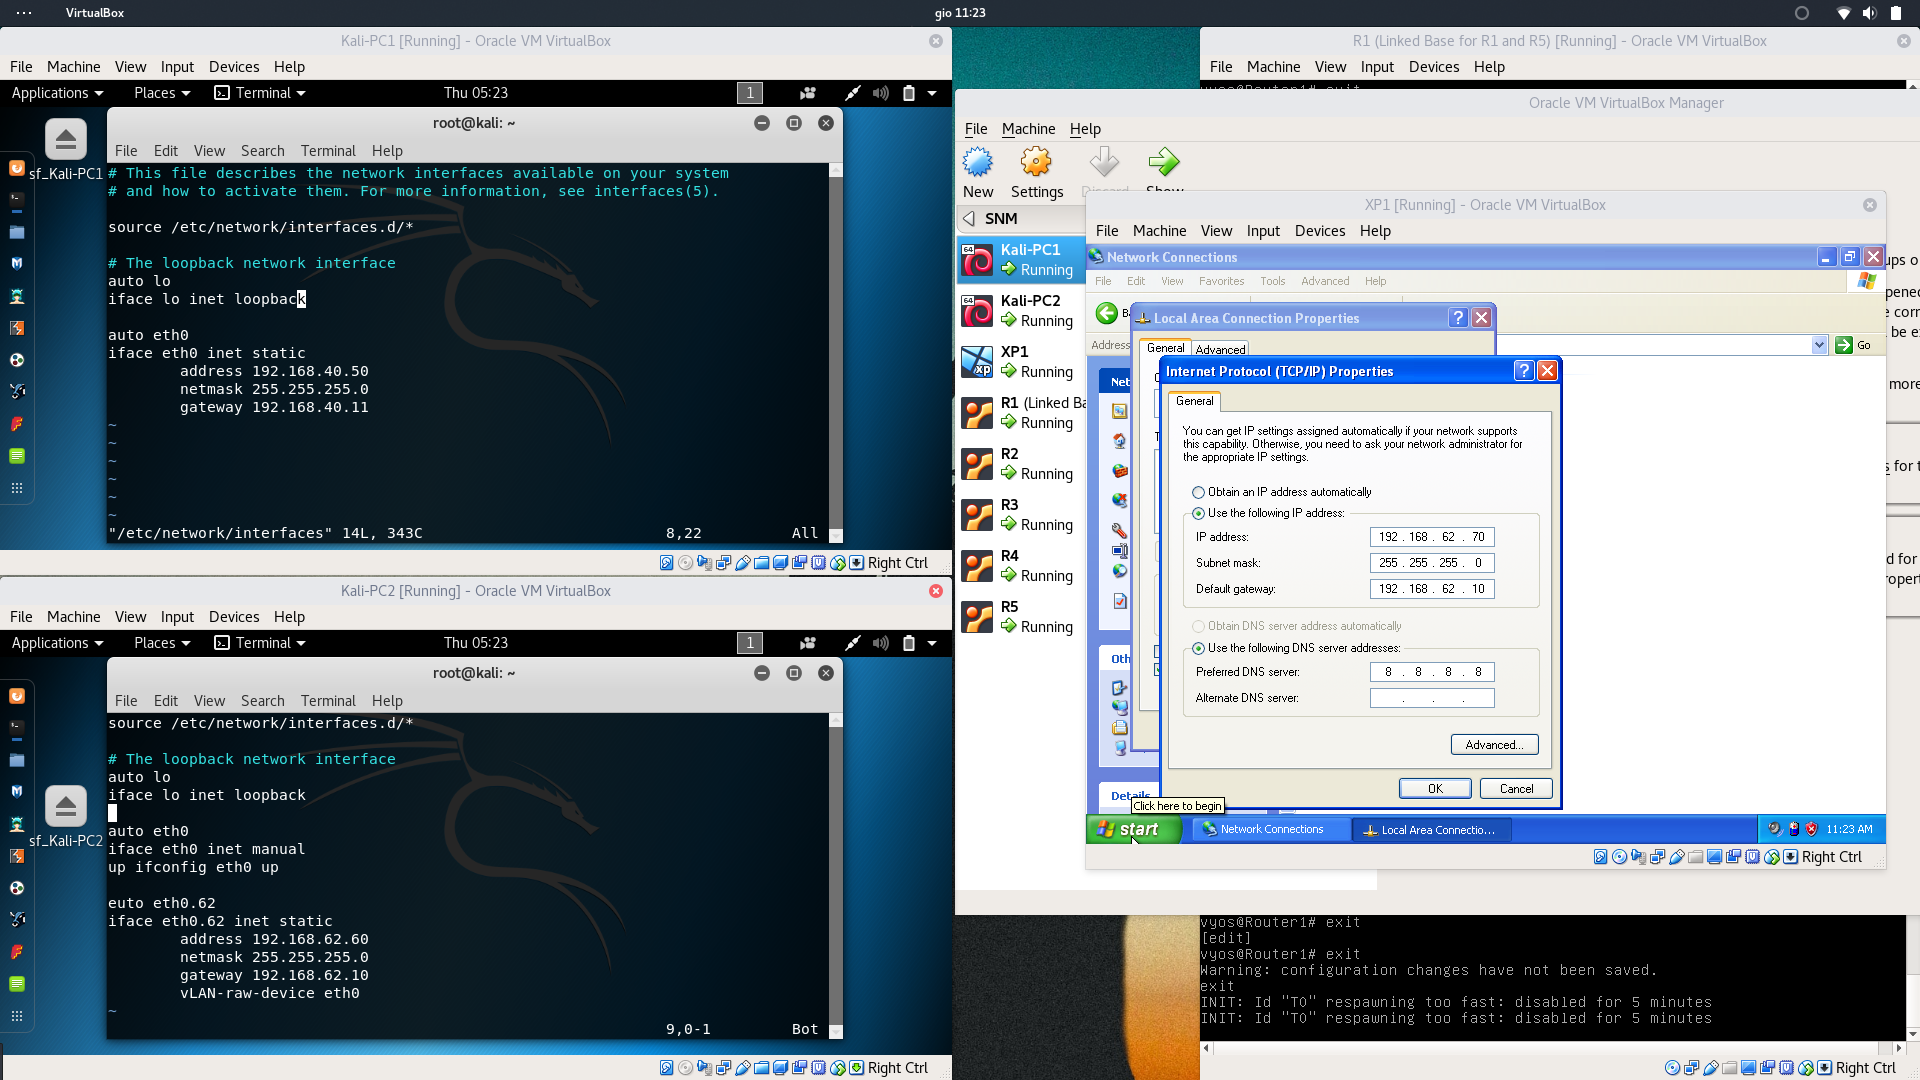
\includegraphics[height=7cm]{img/GlobalConfiguration.png}\par
\end{center}

\subsection{Devices Configuration}

\subsubsection*{R5}
The Router5 is a clone of the Router1.
The network of this router is composed by two enabled adapters:
\begin{itemize}
	\item Adapter 1: Internal Network (Name: intnet);
	\item Adapter 2: NAT Network (Name: NatNetwork).
\end{itemize}
After the start of the machine it is setted with this commands:

\lstinputlisting[language=bash]{cfg_files/r5.txt}

\subsubsection*{R1}
\lstinputlisting[language=bash]{cfg_files/r1.txt}

\subsubsection*{R2}
\lstinputlisting[language=bash]{cfg_files/r2.txt}

\subsubsection*{R3}
\lstinputlisting[language=bash]{cfg_files/r3.txt}

\subsubsection*{R4}
\lstinputlisting[language=bash]{cfg_files/r4.txt}

\subsubsection*{Kali-PC1}
\lstinputlisting[language=bash]{cfg_files/Kali-PC1_interfaces.txt}
\begin{lstlisting}
echo "nameserver 8.8.8.8" >> /etc/resolv.conf
\end{lstlisting}

\subsubsection*{Kali-PC2}
\lstinputlisting[language=bash]{cfg_files/Kali-PC2_interfaces.txt}
\begin{lstlisting}
echo "nameserver 8.8.8.8" >> /etc/resolv.conf
\end{lstlisting}

\subsubsection*{XP1}
% TODO the pic with the DNS setted
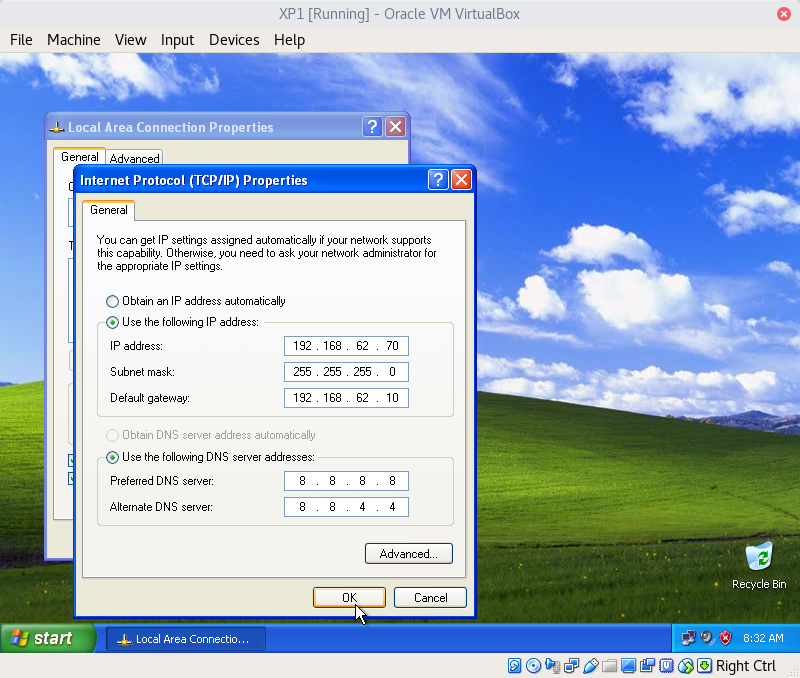
\includegraphics[height=7cm]{img/WinXPNetworkConfiguration.png}\par
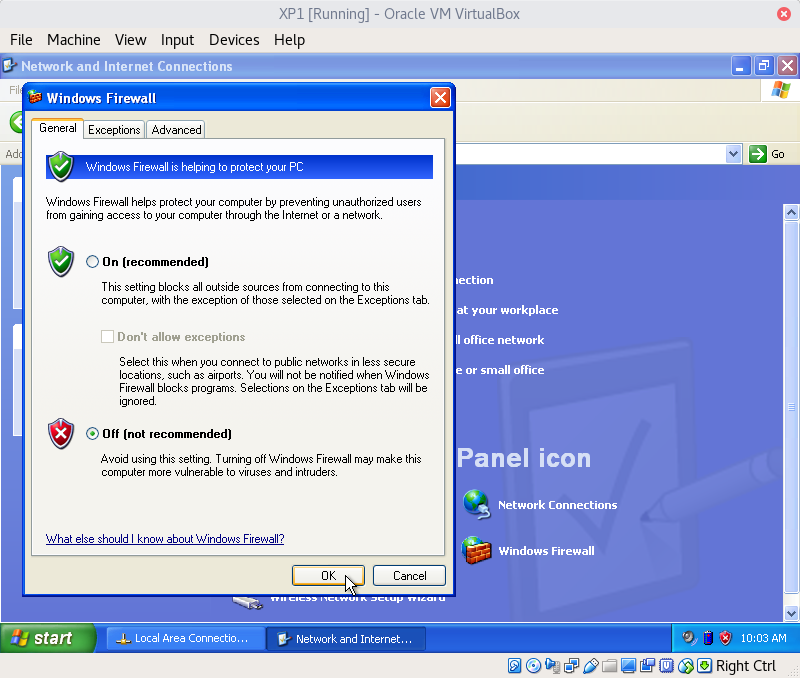
\includegraphics[height=7cm]{img/WinXPFirewallDisabled.png}\par

\subsection{Test to the configuration}
Bash version of a test.\par
\lstinputlisting{scapy/TestConfiguration.sh}
Now it's presented a scapy program used to test if the network was working properly before the attacks.\par
\lstinputlisting{scapy/TestConfiguration.py}

% Section of the Reconnaissance attacks
\section{Reconnaissance Attacks}
% inport recoinnaissance attacks to the document
%% Sample of a report for an attack as requested at wednesday, 5 December 2018, mail "Assignemnt Lab 19"
\subsection{Attack Name}
% Configuration used
\subsubsection*{Configuration used}
% Configuration here
% End of a line -> \\
% End of a paragraph -> \par

% SCAPY program
\subsubsection*{SCAPY program}
%\lstinputlisting{scapy/AttackNameCommentedScapyProgram.py}

% Wireshark presenting  the attacker's messages
\subsubsection*{Attacker's messages}
%\includegraphics[height=7cm]{img/AttackNameWiresharkPacketsCaptured.png}

% Explanation of the result of the attack
\subsubsection*{Attack's result}


% Method recommended to protect the Network against such an attack
\subsubsection*{How to protect the network}


% Sample of a report for an attack as requested at wednesday, 5 December 2018, mail "Assignemnt Lab 19"
\subsection{IP Spoofing}
% Introduction about this attack
\subsection{Introduction}
In order to hide the IP address of a sender machine and at the same time identifying a station active on the network, an attacker could be use a method named \textit{IP spoofing}.\par
The IP spoofing consists to send ICMP packets with a fake source IP that isn't mapped on the network to recognize the reply of the active host connected to the network.\par

% SCAPY program
\subsubsection{SCAPY program}
In this scapy program the attacker has an IP that is not in the network (192.168.102.102) and it sends ICMP packets to all the host that could be present in the subnetwork 192.168.62.0/24.\par
\lstinputlisting{scapy/IPSpoofing.py}

% Wireshark presenting  the attacker's messages
\subsubsection{Attacker's messages}
%Wireshark filter: \textit{icmp \&\& ip.addr == 192.168.102.102}\par
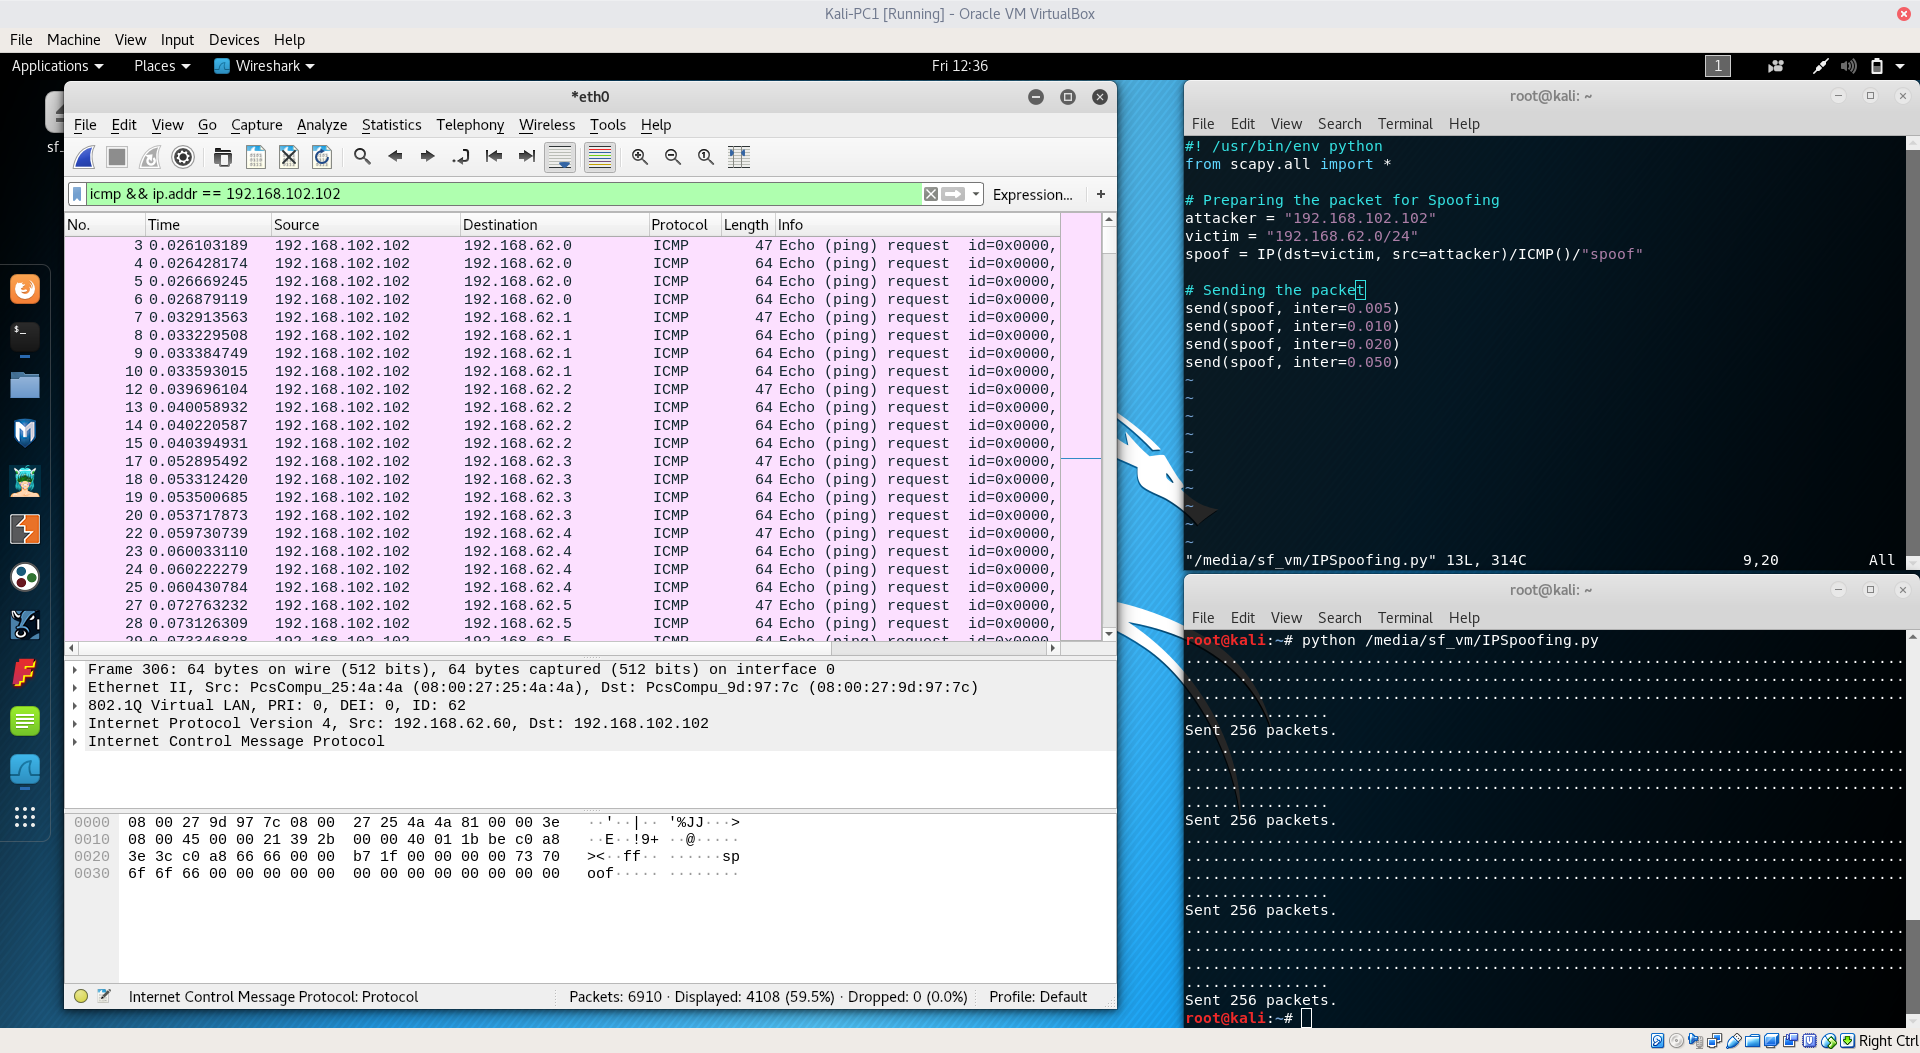
\includegraphics[width=16cm]{img/IPSpoofingICMP.png}

% Explanation of the result of the attack
\subsubsection{Attack's result}
Wireshark has received the ICMP reply packets of the host attacked. So the attacker had sent packets to the active host and the host hadn't recognized the real sender (the attacker).\par
%Wireshark filter: \textit{icmp.type == 0 \&\& ip.addr == 192.168.102.102}\par
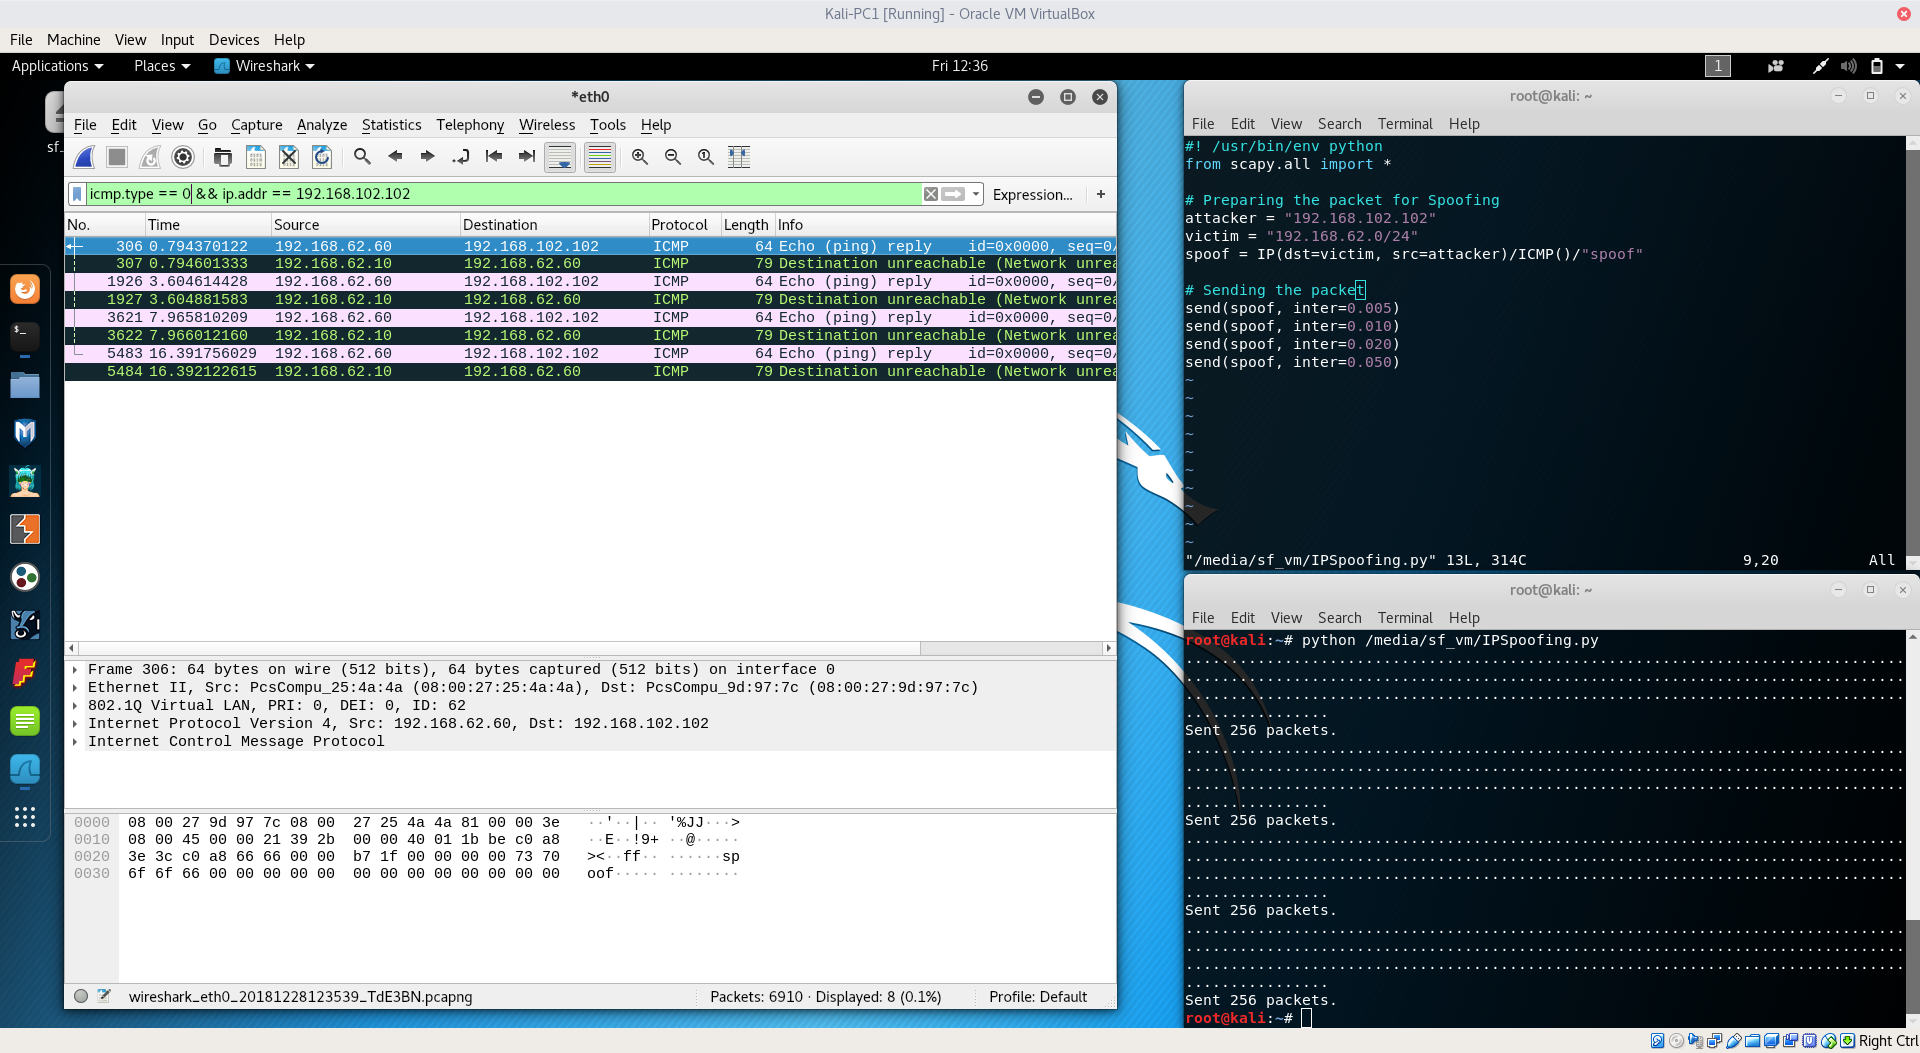
\includegraphics[width=16cm]{img/IPSpoofingReply.png}

% Method recommended to protect the Network against such an attack
\subsubsection{How to protect the network}
In order to protect the network a possible solution is to blocks all the incoming ICMP packets.

% Sample of a report for an attack as requested at wednesday, 5 December 2018, mail "Assignemnt Lab 19"
\subsection{No Flags Set}
% Introduction about this attack
\subsubsection{Introduction}
The TCP protocol isn't permit message with no flags setted.\\
Any operating systems reply to that message in a specific manner. So the attacker could retrive some information about it.\par

% SCAPY program
\subsubsection{SCAPY program}
\lstinputlisting{scapy/NoFlagsSet.py}

% Wireshark presenting  the attacker's messages
\subsubsection{Attacker's messages}
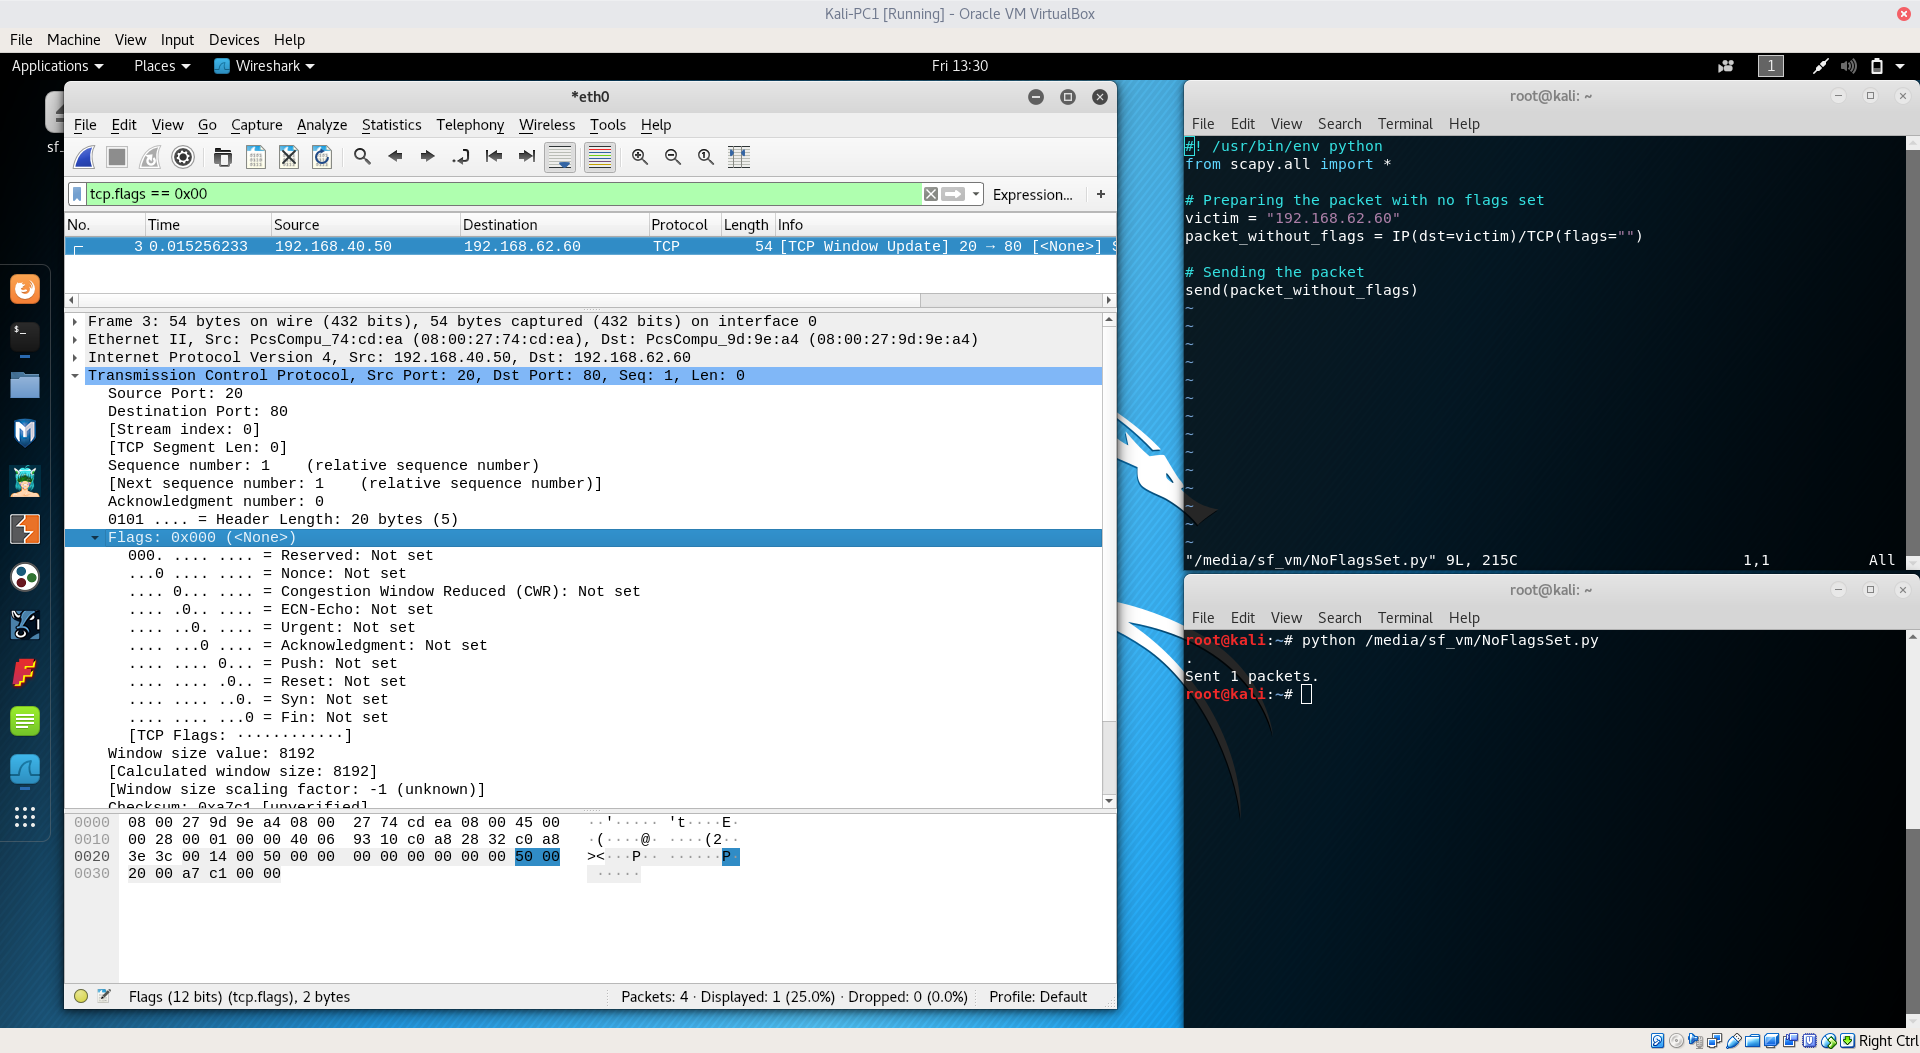
\includegraphics[width=16cm]{img/NoFlagsSetAttackerMessage.png}\par

% Explanation of the result of the attack
\subsubsection{Attack's result}
The host had replyed to the attacker as agreed to its operating system.\\
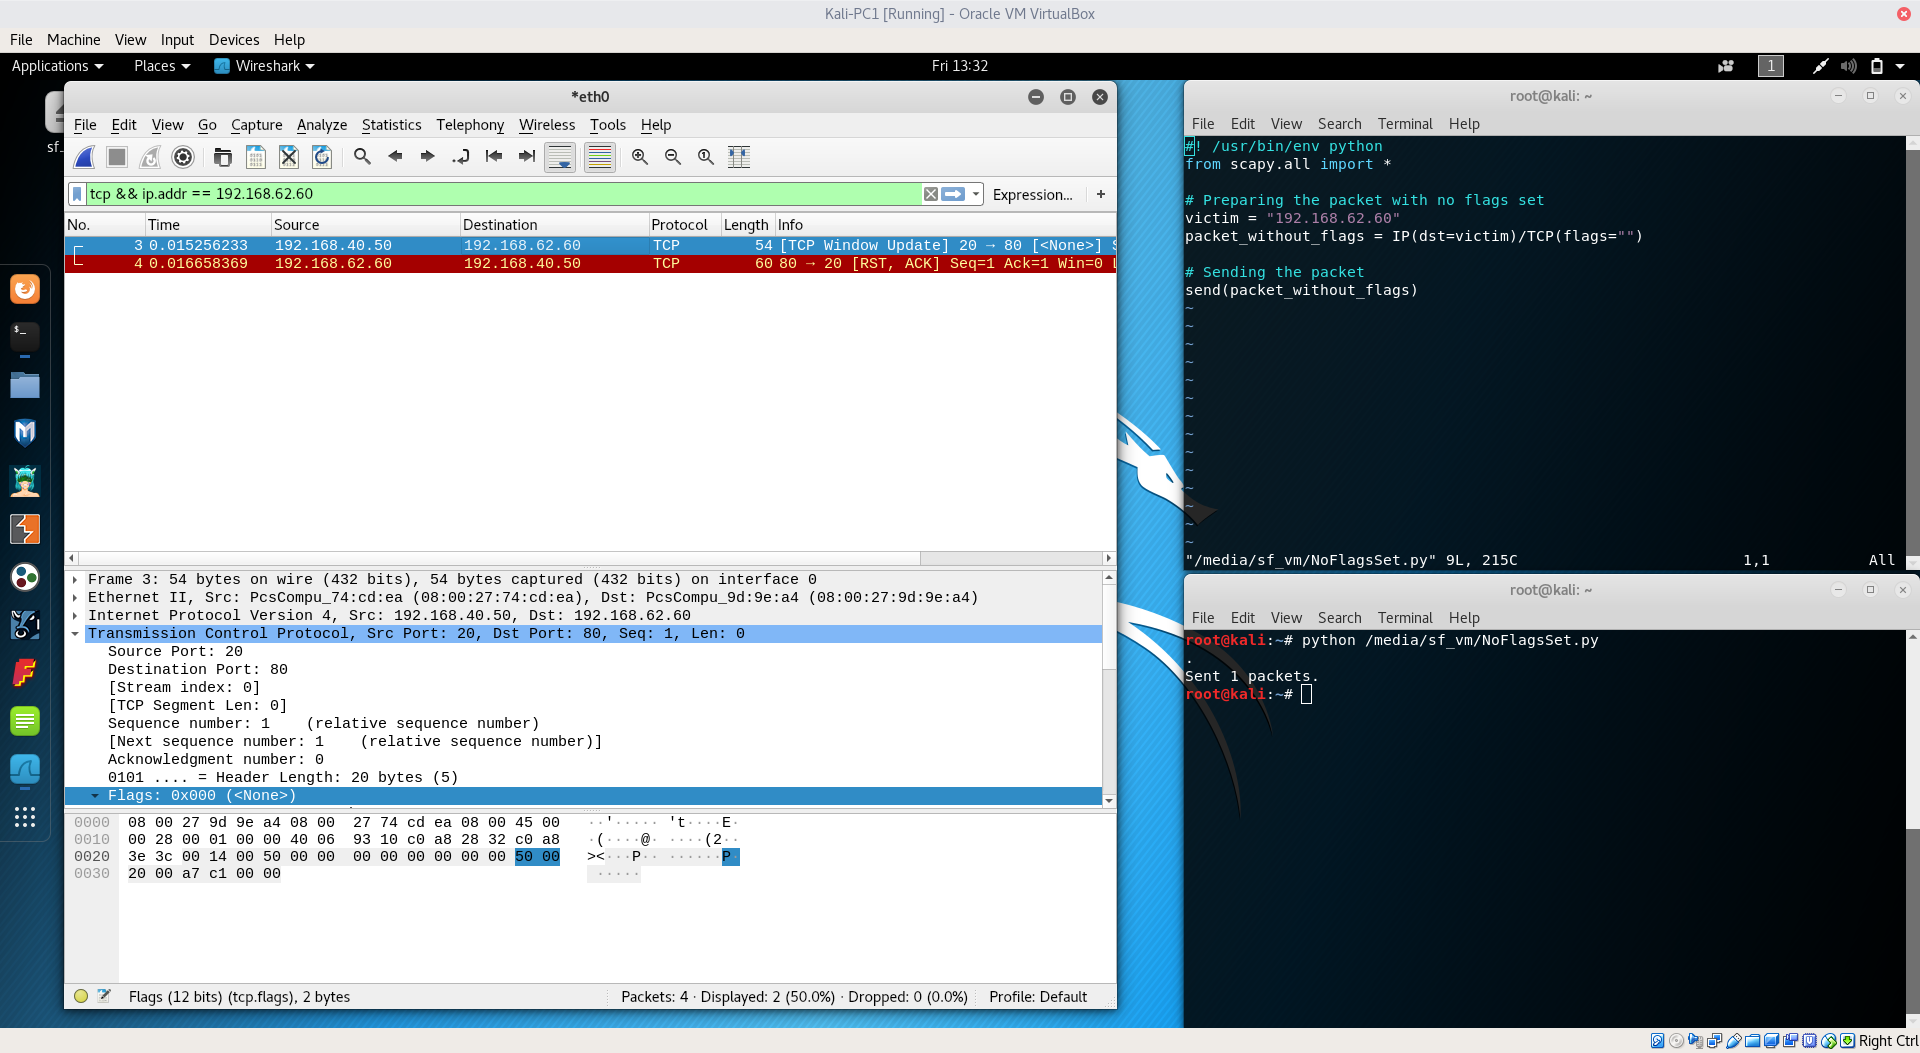
\includegraphics[width=16cm]{img/NoFlagsSetResult.png}\par


% Method recommended to protect the Network against such an attack
\subsubsection{How to protect the network}
In order to protect the victim it could be useful to reject the tcp message with no flags set.


% Section ot the Dos attacks
\section{DoS Attacks}
% inport DoS attacks to the document
% Sample of a report for an attack as requested at wednesday, 5 December 2018, mail "Assignemnt Lab 19"
\subsection{ICMP Redirect}
% Introduction about this attack
\subsubsection{Introduction}
Routers send ICMP Redirect packet to host for conveing new routing information to hosts.\\
This attack uses malformed ICMP Redirect packet to try to change the routing table of a victim.\par

% SCAPY program
\subsubsection{SCAPY program}
\lstinputlisting{scapy/ICMPRedirect.py}

% Wireshark presenting  the attacker's messages
\subsubsection{Attacker's messages}
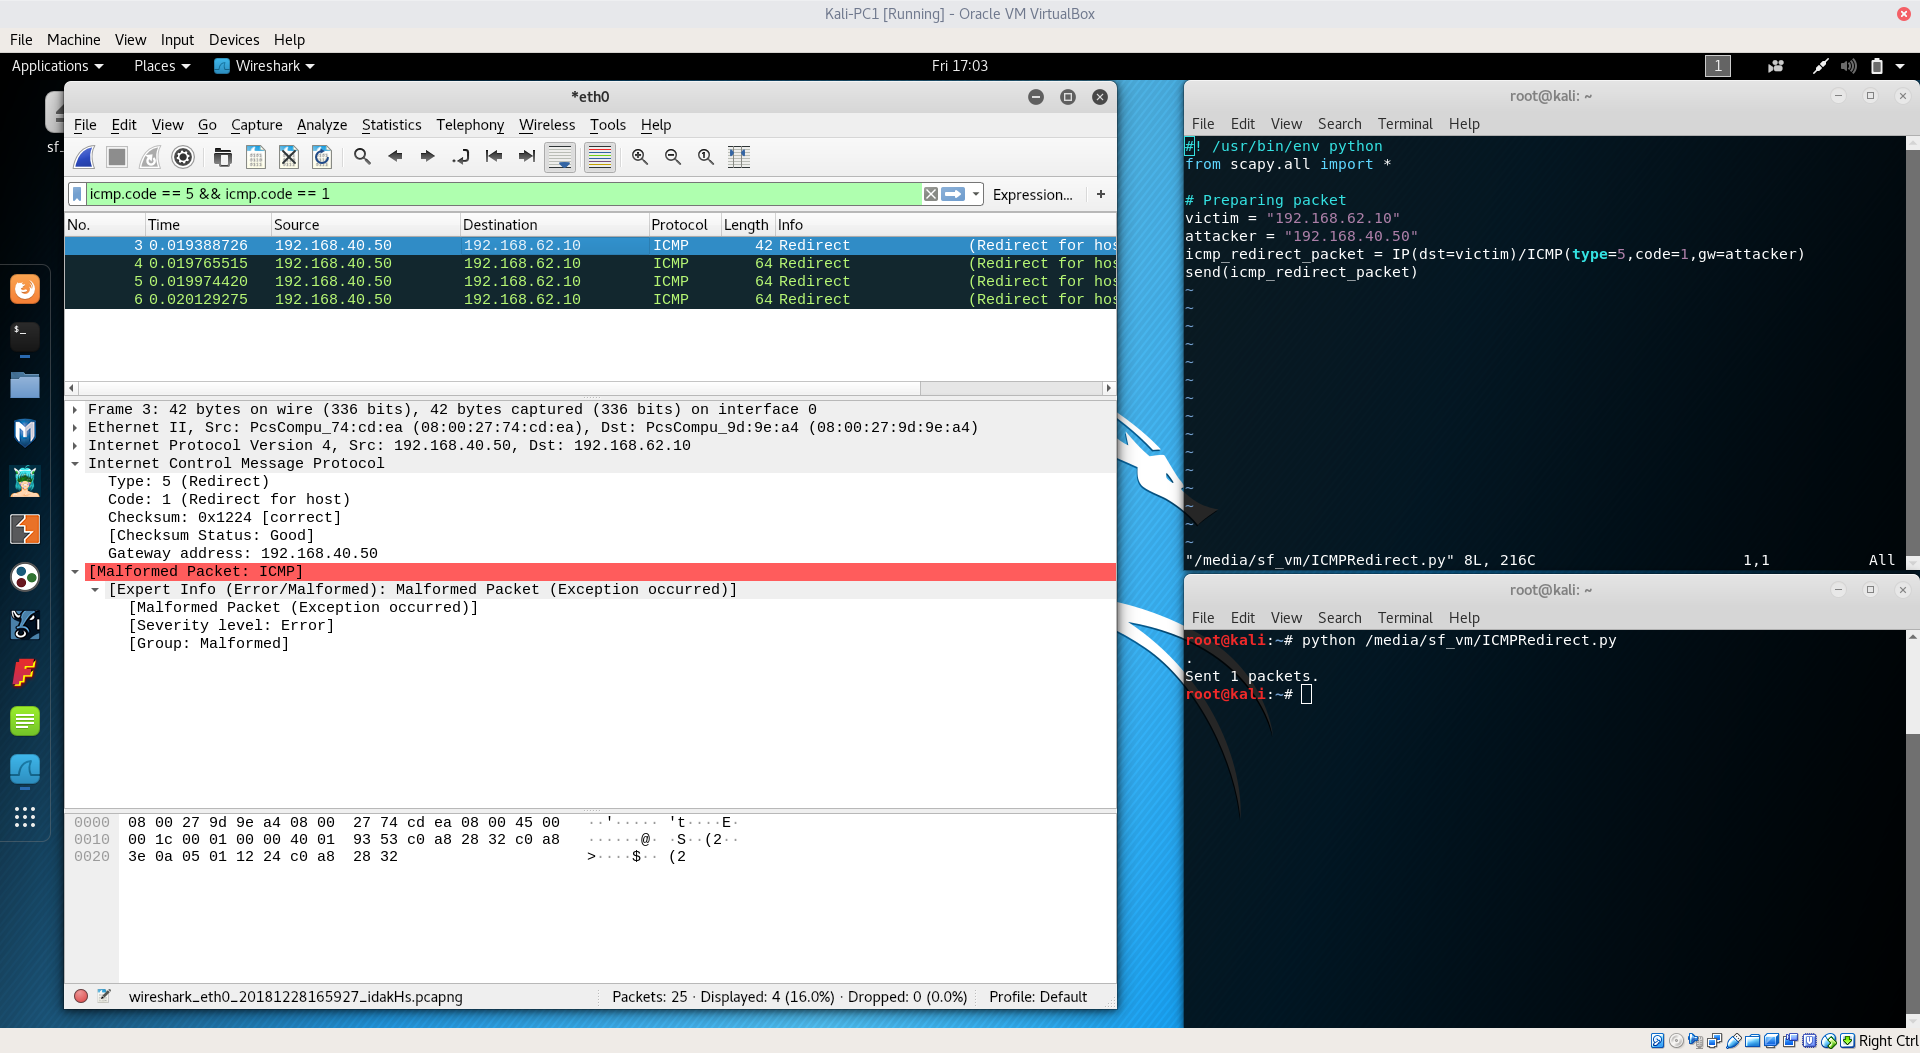
\includegraphics[width=16cm]{img/ICMPRedirect.png}

% Explanation of the result of the attack
\subsubsection{Attack's result}
The aim of this attack is to redirect the traffic to the attacker PC, so the scapy program is set to send a malformed ICMP redirect packet to the victim.

% Method recommended to protect the Network against such an attack
\subsubsection{How to protect the network}
In order to avoid this situation it could be useful block all ICMP packets on routers and hosts if not really needed as is in ordinary situation.

% Sample of a report for an attack as requested at wednesday, 5 December 2018, mail "Assignemnt Lab 19"
\subsection{Ping of Death}
% Introduction about this attack
\subsubsection{Introduction}
An IP packet has a maxiumum length of \textit{65535 bytes} $(2^{16}-1)$ as described in the relative \href{https://tools.ietf.org/html/rfc791}{RFC 791}.\\
So it's not possible to send an IP packet that has a length more larger than that length, but it is possible to send the packet fragmented in plus that one.\\
The receiver could be crash reassembling the packet.\par

% SCAPY program
\subsubsection{SCAPY program}
\lstinputlisting{scapy/PingOfDeath.py}

% Wireshark presenting  the attacker's messages
\subsubsection{Attacker's messages}
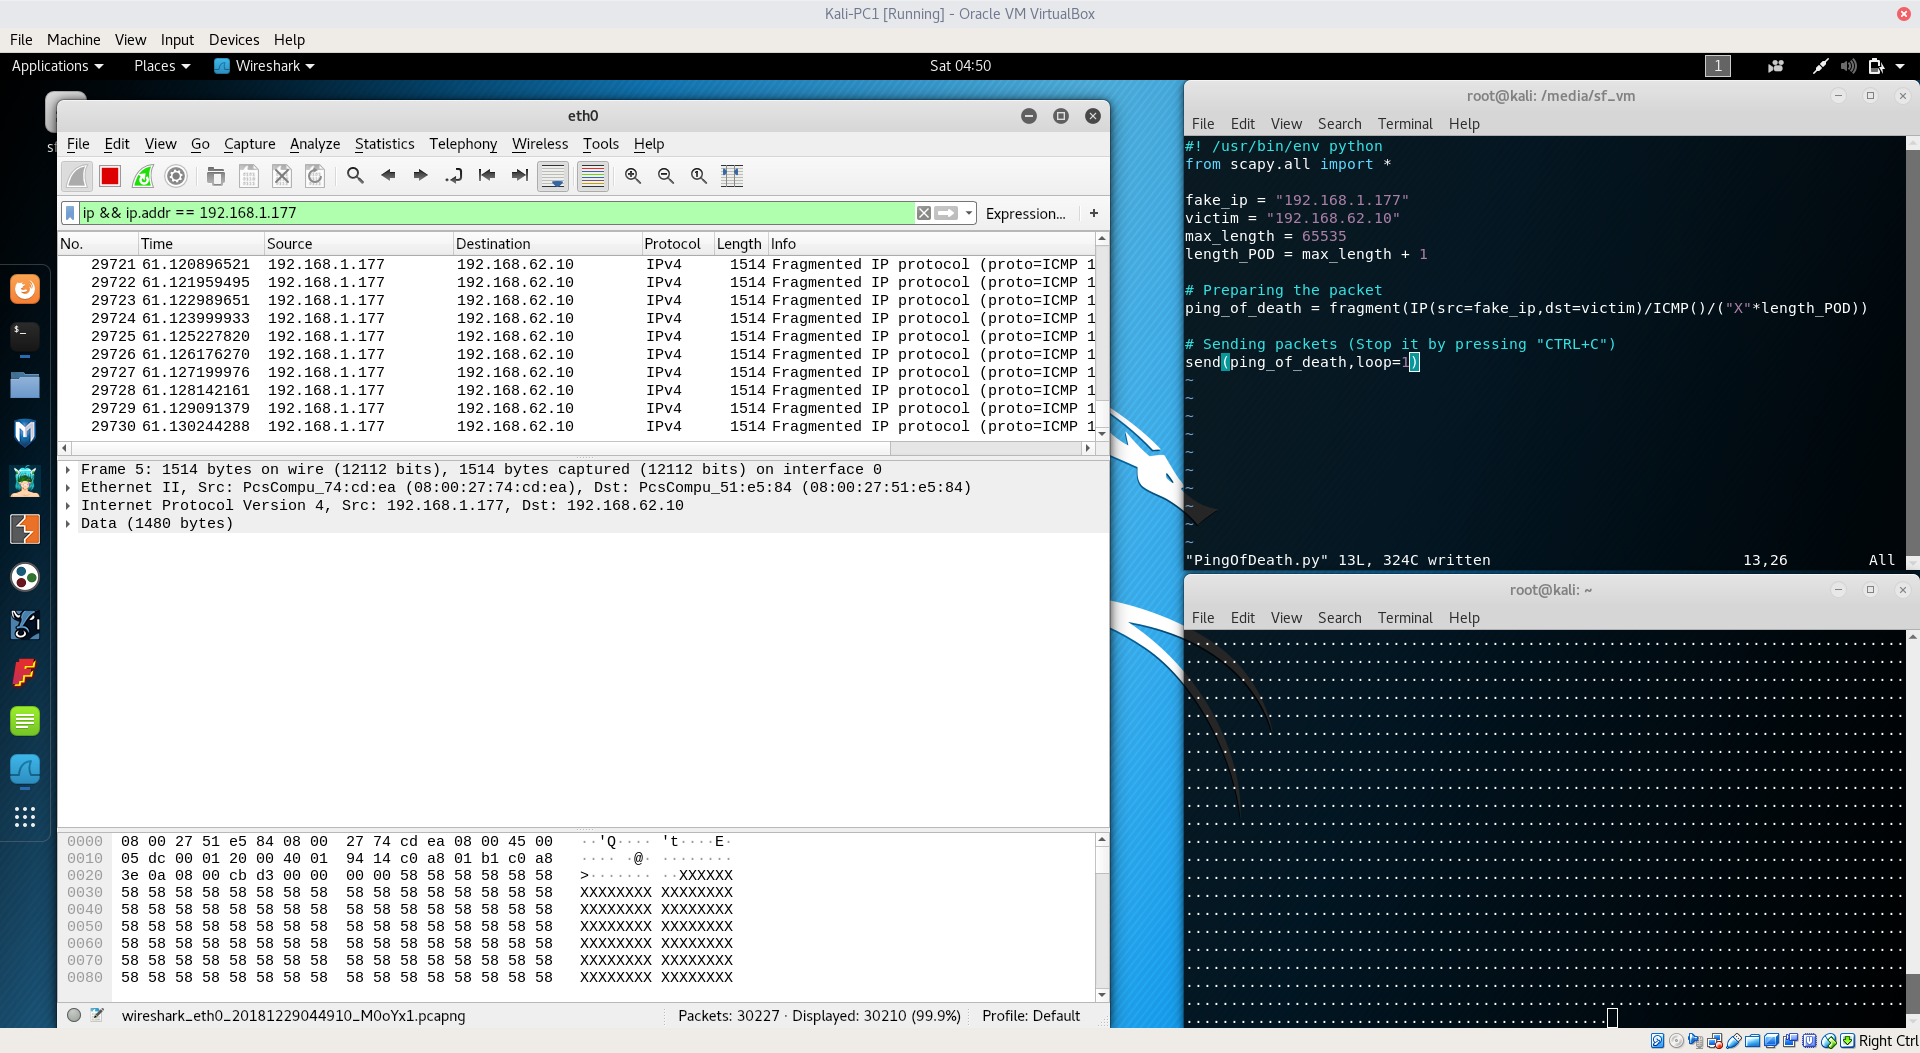
\includegraphics[width=16cm]{img/PingOfDeath.png}

% Explanation of the result of the attack
%\subsubsection{Attack's result}


% Method recommended to protect the Network against such an attack
\subsubsection{How to protect the network}
In order to avoid this attack it could be useful check all incoming IP fragment to recognize if the sum of the "fragment offset" and the "total length" of the IP packet is regular. If not the packet it could be considered invalid and so it could be rejected.\par


% Licence
\vspace*{\fill}
\centering
\tiny{This work is licensed under the Creative Commons Attribution-ShareAlike 4.0 International License. To view a copy of this license, visit \href{http://creativecommons.org/licenses/by-sa/4.0/}{http://creativecommons.org/licenses/by-sa/4.0/} or send a letter to Creative Commons, PO Box 1866, Mountain View, CA 94042, USA.}

\end{document}
